%! TEX root = ../outline.tex

% \subsection{Gradient Boosted Regression Trees}

\begin{figure}[H]%
    \centering
    \subfloat[$\tau = 0.5$.]{{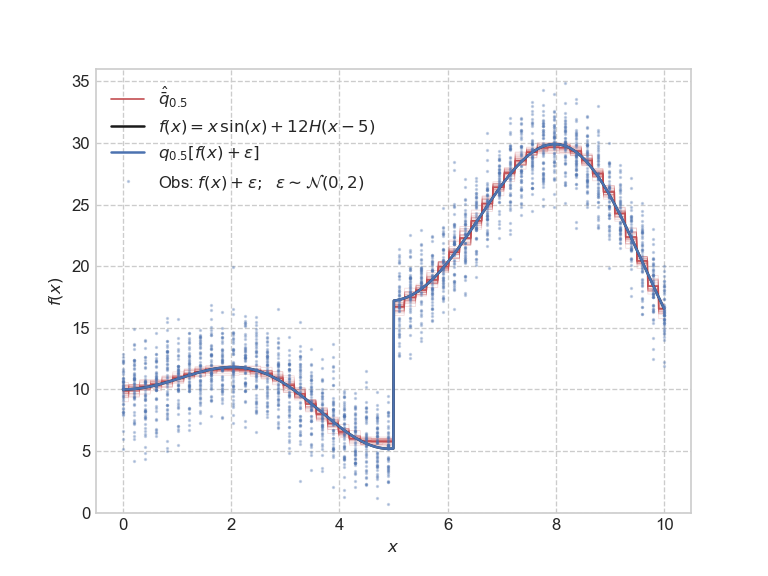
\includegraphics[width=0.53\linewidth]{figs/grad_boost/1d_boosted_regression_quantile_ex_0_5} }}\hspace*{-1.0em}%
    \subfloat[$\tau = 0.9$.]{{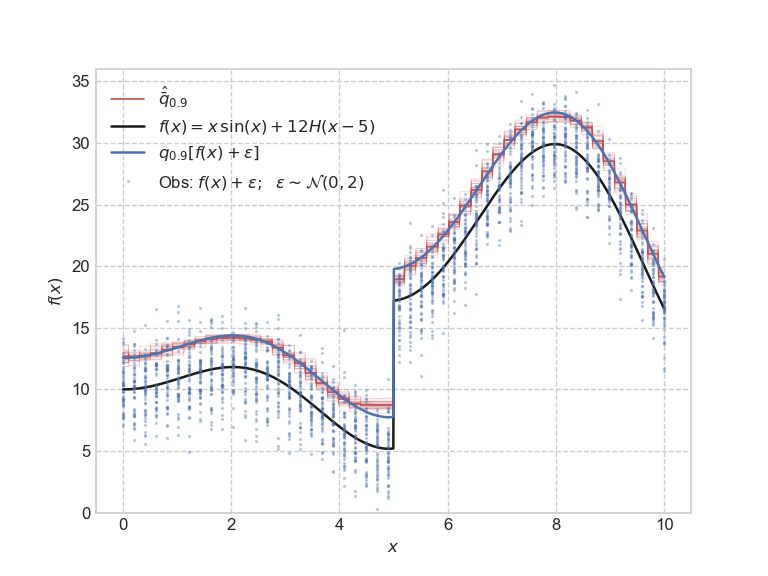
\includegraphics[width=0.53\linewidth]{figs/grad_boost/1d_boosted_regression_quantile_ex_0_9} }}\hspace*{-1.0em}%
    \\
    \subfloat[$\tau = 0.75$.]{{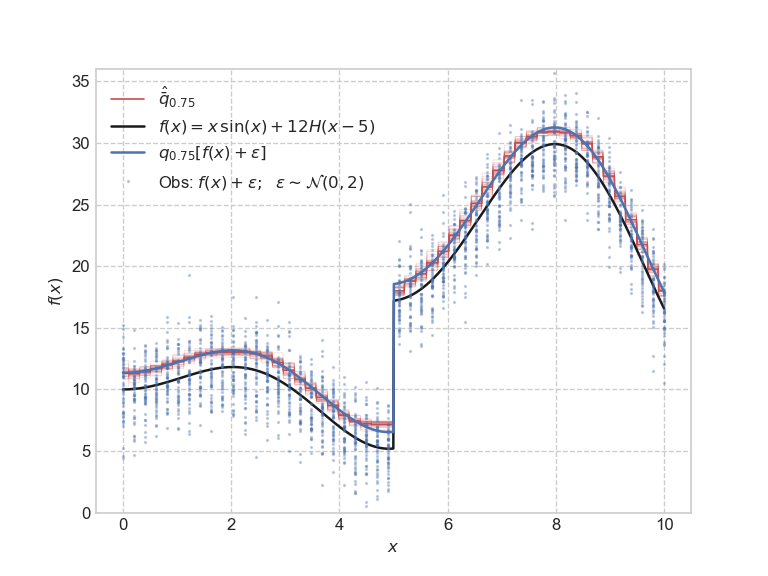
\includegraphics[width=0.53\linewidth]{figs/grad_boost/1d_boosted_regression_quantile_ex_0_75} }}\hspace*{-1.0em}%
    \subfloat[$\tau = 0.95$.]{{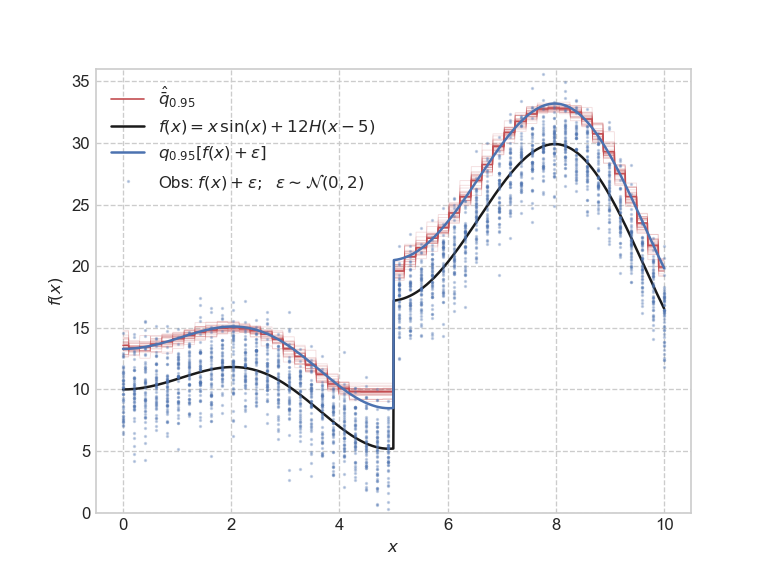
\includegraphics[width=0.53\linewidth]{figs/grad_boost/1d_boosted_regression_quantile_ex_0_95} }}\hspace*{-1.0em}%
    \caption[Gradient boosted quantile regression example.]{Gradient boosted quantile regression example.}%
    \label{fig:gb1}%
\end{figure}

Two candidate gradient boosting implementations were evaluated for use in this work.  A test problem was constructed to check that the standard gradient boosting regression technique is resilient to discontinuities in the data since the response fields are expected to abruptly change when moving across a spacer grid.  The function $y = x \mathrm{sin}(x) +12 \mathcal H(x-5)+\varepsilon$ with $x\in [0,10]$ was used for testing.  $\mathcal H$ denotes the Heaviside function. Synthetic noise, $\varepsilon \sim \mathcal N(0,2)$, was applied to the piecewise smooth test function.   5000 total samples were drawn from the test function. The test data was spatially aggregated to 100 axial levels to mimic CTF axial grid spacing.  Four separate quantile regressors ($\tau = \{0.5, 0.75, 0.9, 0.95 \})$ were then fit to the data by algorithm \ref{alg:boosting}. The predicted quantiles, conditioned on $x$, were compared to the expected results, as shown in figure \ref{fig:gb1}. For this problem results from the scikit-learn gradient boosting implementation are compared to a custom boosting implementation, named $pCRTree$, developed specifically to solve the classification and quantile regression problems in this work.  The residuals provided figure \ref{fig:gb2} show that the custom implementation performs similarly to the well-tested scikit-learn implementation with both models agreeing with the theoretical large-sample quantile distributions provided by equation \ref{eq:theory_qdist_1}.

\begin{figure}[H]%
    \centering
    \subfloat[$\tau = 0.5$ model residuals.]{{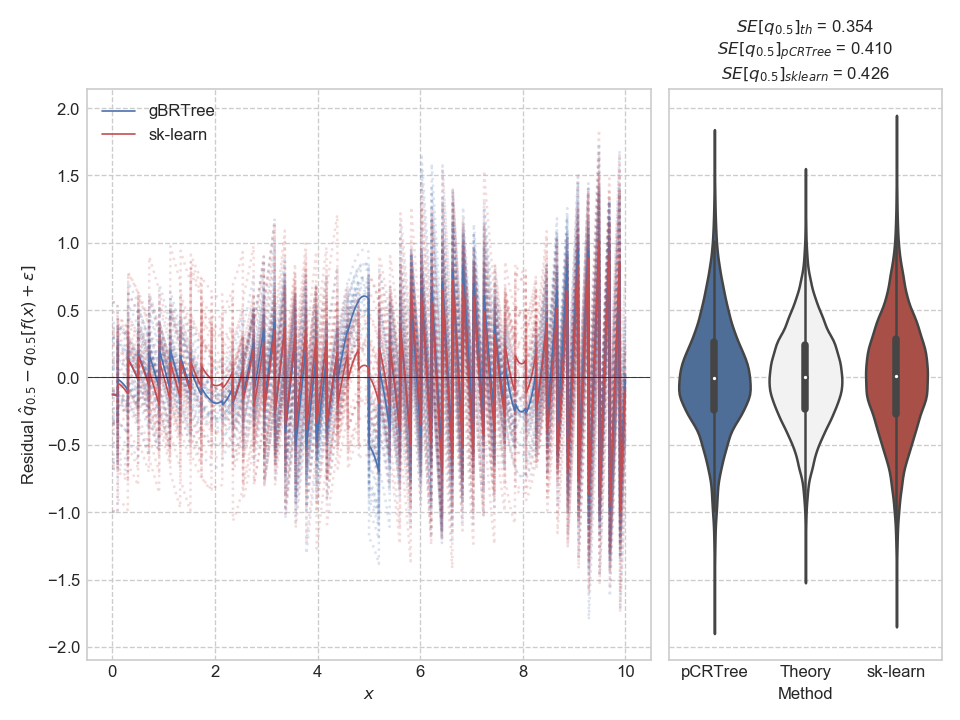
\includegraphics[width=0.53\linewidth]{figs/grad_boost/1d_boosted_regression_quantile_resid_0_5} }}\hspace*{-1.0em}%
    \subfloat[$\tau = 0.9$ model residuals.]{{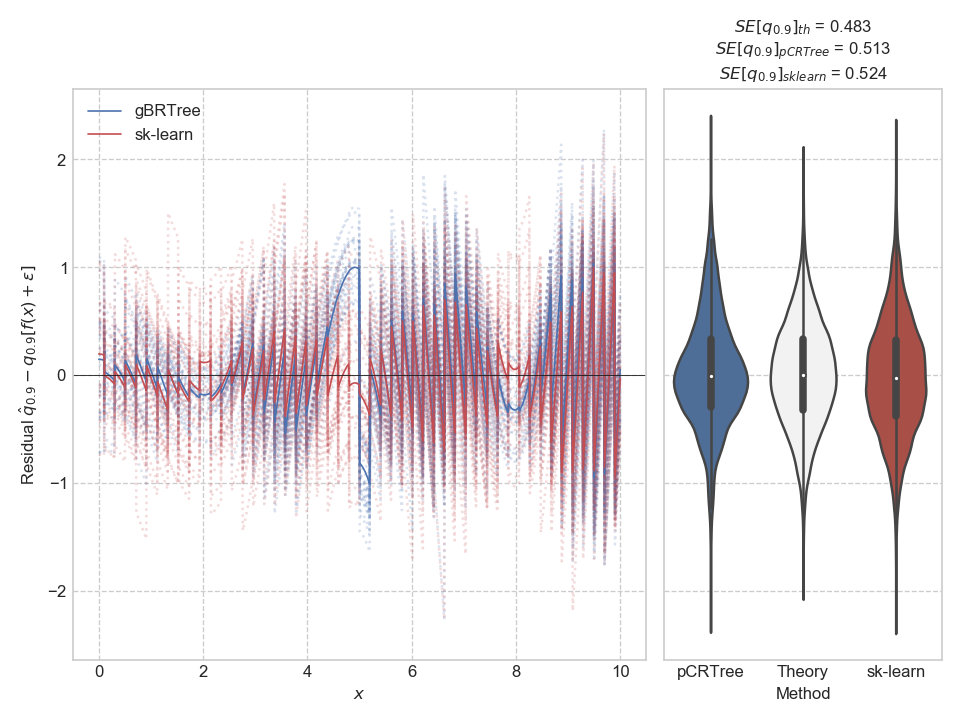
\includegraphics[width=0.53\linewidth]{figs/grad_boost/1d_boosted_regression_quantile_resid_0_9} }}\hspace*{-1.0em}%
    \\
    \subfloat[$\tau = 0.75$ model residuals.]{{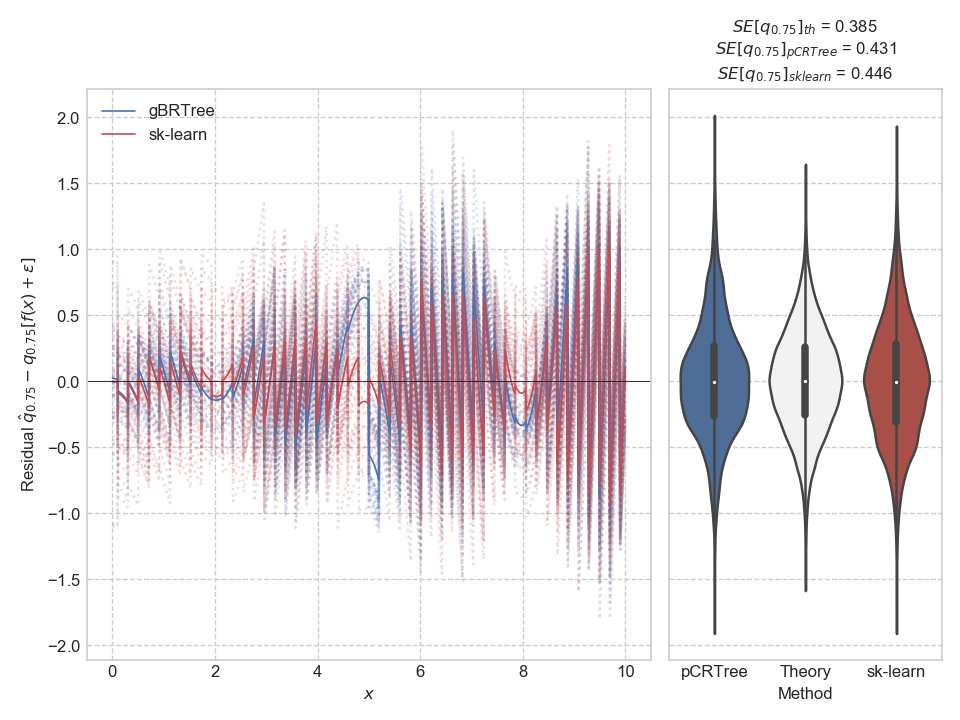
\includegraphics[width=0.53\linewidth]{figs/grad_boost/1d_boosted_regression_quantile_resid_0_75} }}\hspace*{-1.0em}%
    \subfloat[$\tau = 0.95$ model residuals.]{{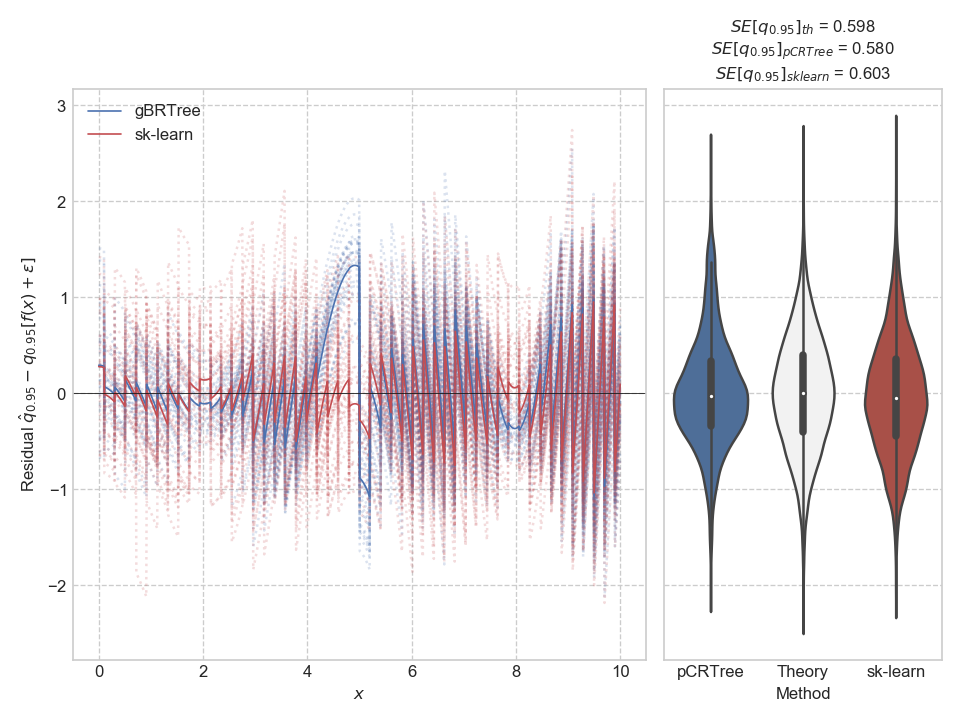
\includegraphics[width=0.53\linewidth]{figs/grad_boost/1d_boosted_regression_quantile_resid_0_95} }}\hspace*{-1.0em}%
    \caption[Gradient boosted quantile regression residual summary.]{Gradient boosted quantile regression residual summary.  The theoretical residual distribution were computed according to equation \ref{eq:theory_qdist_1}.} %
    \label{fig:gb2}%
\end{figure}

The parametric copula family which corresponds to a given set of local core conditions must also be determined in order to fully specify the copula required in the definition of the joint density function given in equation \ref{eq:simple_vine_model}.   This gives rise to a typical supervised classification problem which will be solved using the gradient boosting method.  The family of copula, $\mathbf \Theta_c$, i.e. either Frank, Clayton, or Gumbel, should be determined by the classifier provided a local core thermal hydraulic state vector $\mathbf p$.   The gradient boosted classification algorithm can be recovered by substituting the exponential loss function shown in equation \ref{eq:exploss} into algorithm \ref{alg:boosting}.   

\begin{align}
L(y, F(\mathbf p)) &= \E \left[ e^{-yF(\mathbf p)}\right] \nonumber \\
 &= \frac{1}{N}\sum_i^N e^{-y_iF(\mathbf p_i)}
\label{eq:exploss}
\end{align}
Where $y$ takes on integer values in $\{-1, 1\}$ for the classification problem.

A two-class test case was devised to validate the custom boosting implementation against the scikit-learn implementation.   This is meant as a demonstration for qualitative understanding of the boosted classification algorithm output.  In this problem red and blue points were emplaced in a two dimensional space as shown in figure \ref{fig:gb3}.  These predefined points form the necessary training data for the test problem. The goal of this test is to segregate the input space, $\{x, y\}$, into regions which are most likely to contain only one color of points. Results from the test 2-D classification test problem are shown in the figure.   In much the same way regression trees produce piecewise constant predictions, the boosted classifier partitions the input space by segregating the space along orthogonal splits.  

Classifier predictions are made by tallying the weighted predictions of each constituent fitted classification weak learner (CART tree) in the boosted model.  By tallying the predictions of all trees in the model one can obtain a probability mass function over all possible classes.  The probability mass function is visualized in figure \ref{fig:gb3}(b) wherein the predicted probability of the ``blue'' class obtained from the fitted boosted model is shown. The most likely class at each requested point is taken as the output of the classification model.

\begin{figure}[H]%
    \centering
    \subfloat[Class predictions.]{{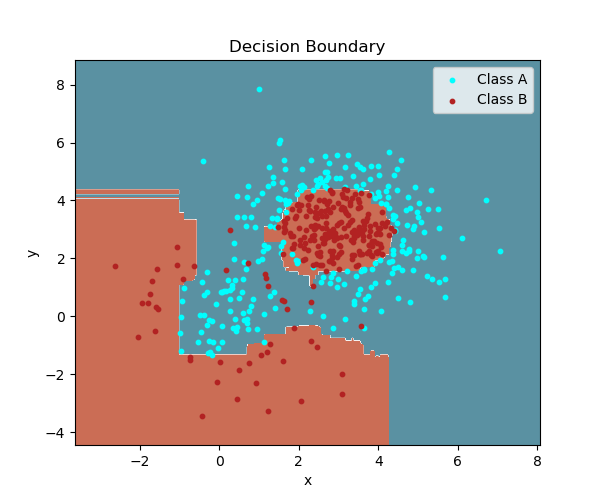
\includegraphics[width=0.50\linewidth]{figs/grad_boost/dblgauss_boosted_classify_ex} }}\hspace*{-1.0em}%
    \subfloat[Blue class probability.]{{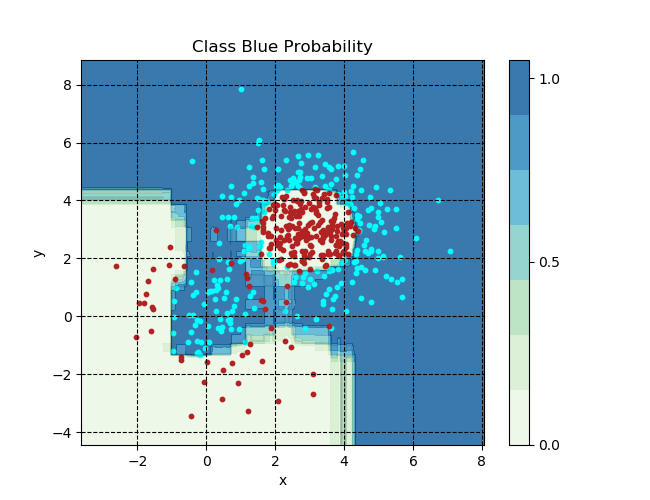
\includegraphics[width=0.54\linewidth]{figs/grad_boost/dblgauss_boosted_classify_probs} }}%
    \caption{Two-class gradient boosted classifier example.}%
    \label{fig:gb3}%
\end{figure}

Finally, gradient boosting can be used to estimate the relative explanatory power of each predictive variable included in the model.  This is done by tallying the number of times a particular dimension is split upon in the CART fitting process and weighting these splits by a gain measure.  The gain can be interpreted as the benefit of making a particular split in the decision tree as measured by improvement in $R^2$ for regression problems, or improvement in class purity as measured by the Gini impurity ratio for classification problems.  Finally, a weighted sum of the split gains of each tree is performed over all boosted iterations to obtain relative variable importances. Friedman provides a detailed explanation of this relative variable importance computation \cite{friedman2001}.  This ability of gradient boosting to identify important predictors has been exploited in email filter and web page ranking applications \cite{chapelle2011}, \cite{Tyree2011}.  In the case of copula prediction, exogenous variables which are extraneous can be detected and eliminated from the model to save computation time.  
%The ability to identify unimportant features is demonstrated in section \ref{sec:feature_eng} in figure \ref{fig:ktauregfeatureimp}.
